\documentclass[journal,twoside,web]{ieeecolor}
\usepackage{tmi}
\usepackage{booktabs}
\usepackage{cite}
\usepackage{amsmath,amssymb,amsfonts}
\usepackage{algorithmic}
\usepackage{graphicx}
\usepackage{siunitx}
\usepackage{textcomp}

\usepackage{xcolor}

\makeatletter
\let\NAT@parse\undefined
\makeatother
\usepackage{hyperref}

\usepackage[capitalise,noabbrev]{cleveref}


\def\BibTeX{{\rm B\kern-.05em{\sc i\kern-.025em b}\kern-.08em
	T\kern-.1667em\lower.7ex\hbox{E}\kern-.125emX}}
\markboth{\journalname, VOL. XX, NO. XX, XXXX 2024}
{Tan \MakeLowercase{\textit{et al.}}: DeepDWI}


\newcommand{\argmin}{\operatornamewithlimits{argmin}}
\newcommand{\norm}[1]{\left\lVert#1\right\rVert}


% FK:
% 1. start with problem statement
% 2. current solution and limitation
%
% Blackbox is not in favor

\begin{document}
	\title{Diffusion-Weighted Imaging with Learned Nonlinear Latent Space Modeling and Self-Supervised Reconstruction (DeepDWI)}

	\author{Zhengguo Tan, Julius Glaser, Patrick A Liebig, Annika Hofmann, Frederik B Laun, Florian Knoll
		\thanks{This work was supported in part by
			German Research Foundation (DFG)
			under projects 513220538 and 512819079,
			project 500888779 in the Research Unit RU5534
			for MR biosignatures at UHF,
			and by the National Institutes of Health (NIH)
			under grants R01 EB024532 and P41 EB017183.
			In addition, scientific support and HPC resources
			were provided by
			the Erlangen National High Performance Computing Center (NHR)
			of Friedrich-Alexander-University Erlangen-Nuremberg (FAU)
			under the NHR project b143dc.
			NHR is funded by federal and Bavarian state authorities.
			NHR@FAU hardware is partially funded by
			DFG under project 440719683. \textit{(Corresponding Author:~Zhengguo Tan)}}
		\thanks{Z.~Tan was with the Department
			Artificial Intelligence in Biomedical Engineering (AIBE),
			FAU, Erlangen, Germany.
			He is now with
			the Michigan Institute for Imaging Technology and Translation
			(MIITT),
			Department of Radiology,
			University of Michigan, Ann Arbor, MI 48109 USA
			(e-mail: zgtan@med.umich.edu).}
		\thanks{J.~Glaser was with the Department of Medical Engineering,
			FAU, Erlangen, Germany.
			He is now with the Institute of Radiology,
			University Hospital Erlangen,
			FAU, Erlangen, Germany
			(e-mail: julius.glaser@fau.de).}
		\thanks{P.~A.~Liebig is with Siemens Healthcare GmbH, Erlangen, Germany
			(e-mail: patrick.liebig@siemens-healthineers.com).}
		\thanks{A.~Hofmann is with the Department AIBE,
			FAU, Erlangen, Germany
			(e-mail: annika.ah.hofmann@fau.de).}
		\thanks{F.~B.~Laun is with the Institute of Radiology,
			University Hospital Erlangen,
			FAU, Erlangen, Germany
			(e-mail: Frederik.Laun@uk-erlangen.de).}
		\thanks{F.~Knoll is with the Department AIBE,
			FAU, Erlangen, Germany
			(e-mail: florian.knoll@fau.de).}
	}

	\maketitle

	% Keep the abstract to 250 words or less.
	\begin{abstract}
		% Define all symbols used in the abstract. Do not cite references in the abstract.
		The code is publicly available at: \url{https://github.com/ZhengguoTan/DeepDWI}.
	\end{abstract}

	\begin{IEEEkeywords}
	Diffusion-weighted imaging, Image reconstruction, Generative AI, Latent space, Self-supervised learning
	\end{IEEEkeywords}

	% ============================== %
	\section{Introduction}
	\label{SEC:INTRO}
	\IEEEPARstart{H}{igh}-dimensional magnetic resonance imaging (HD-MRI)
	has been a flourishing field,
	which refers to the acquisition, reconstruction and analysis of
	multi-dimensional multi-contrast-weighted MRI data.
	Examples of HD-MRI include but are not limited to
	magnetic resonance spectroscopic imaging (MRSI)
	\cite{brown_1982_mrsi},
	diffusion-weighted imaging (DWI)
	\cite{lebihan_1986_diff,merboldt_1985_diff},
	and quantitative parameter mapping
	\cite{doneva_2010_moba,ma_2013_mrf}.
	Conventional HD-MRI, however, necessitates long acquisition,
	resulting in data vulnerable to subject motion
	and system imperfections, as well as high computational burden.
	DWI, in particular, poses challenges in the pursuit of
	high spatial, temporal, and angular resolution.
	DWI is typically acquired via
	the pulsed gradient spin echo sequence \cite{stejskal_1965_pgse}
	followed by fast echo-planar imaging (EPI) readouts
	\cite{mansfield_1977_epi}.
	However, the use of long echo trains in EPI results in
	geometric distortion artifacts and low spatial resolution.
	Plus, the interest in acquiring multiple diffusion directions
	for the improvement of angular resolution and
	for the probe to tissue microstructure increases the scan time.

	Advances in parallel imaging
	\cite{roemer_1990_pi,sodickson_1997_smash,
	pruessmann_1999_sense,pruessmann_2001_gsense,griswold_2002_grappa}
	and compressed sensing
	\cite{lustig_2007_cs,block_2007_cs,liang_2007_psf}
	have enabled accelerated acquisition for HD-MRI.
	In particular, the low-rank model \cite{cai_2010_svt}
	has been a powerful tool in dimension reduction.
	Usually, singular value decomposition (SVD) is used to
	learn a truncated temporal basis function from
	a large-scale physics-informed dictionary
	\cite{huang_2012_t2basis,lam_2014_spice,mcgivney_2014_svdmrf}.
	The temporal basis function is then integrated
	with the MRI forward model,
	i.e.~the sensitivity encoding operator \cite{pruessmann_2001_gsense},
	for joint reconstruction of the corresponding spatial basis images.
	In addition, low-rank regularization can be employed
	in the joint reconstruction \cite{tamir_2017_t2shuffling}.

	Beyond the low-rank technique,
	advanced neural networks, e.g.~autoencoder \cite{hinton_2006_ae},
	have been explored for HD-MRI reconstruction and
	proven to supply more accurate representations of
	high-dimensional data than SVD.
	Lam et al.~\cite{lam_2019_mrsi} and Mani et al.~\cite{mani_2021_qmodel}
	proposed to first learn a denoising autoencoder (DAE) model
	from a physics-informed simulated dictionary
	and then incorporate the learned DAE model as a regularizer
	in the alternating direction method of multipliers (ADMM)
	\cite{boyd_2010_admm}
	unrolling reconstruction.
	Pioneered by Gregor and LeCun \cite{gregor_2010_algunroll},
	algorithm unrolling enables the use of learned deep \textit{prior}
	as regularization and faster inference than
	iterative reconstruction with hand-crafted regularization functions
	\cite{monga_2021_algunroll}.
	Algorithm unrolling has been introduced to
	accelerated MRI reconstruction and
	employed in various scenarios:
	supervised learning with fully sampled reference images
	\cite{hammernik_2018_varnet,aggarwal_2018_modl},
	and self-supervised learning
	with only undersampled data available for training
	\cite{yaman_2020_ssdu,yaman_2022_zs}.
	Noteworthy, it is rather difficult to acquire fully-sampled DWI
	for the training of a regularization functional.
	First, fully-sampled DWI requires a longer echo train in EPI,
	which not only elongates the scan time
	but also increases off-resonance-induced geometric distortion.
	Second, there exists a wide range of diffusion acquisition modes,
	thereby requiring a larger dataset than
	the two-dimensional imaging scenario \cite{knoll_2020_fastmri}.
	Therefore, self-supervised learning is more appropriate
	for DWI reconstruction.

	Deep neural networks are capable of learning
	not only regularization functions,
	but also MR-physics forward operators.
	% Zhu et al.~\cite{zhu_2018_automap} proposed
	% the automated transform by manifold approximation (AUTOMAP),
	% which learns the mapping between the sensor and the image domain
	% for data-driven supervised image reconstruction.
	Liu et al.~\cite{liu_2021_relax} proposed
	the reference-free $T_1$ parameter maps extraction (RELAX)
	self-supervised deep learning reconstruction,
	which learns the mapping from $T_1$ parameter maps to
	undersampled multi-coil multi-contrast $k$-space data.
	Arefeen et al.~\cite{arefeen_2023_latent} proposed
	to replace the conventional SVD-based linear subspace modeling
	\cite{huang_2012_t2basis}
	by the latent decoder model within DAE
	for improved $T_2$-weighted image reconstruction.
	The capability of DAE to learn DWI models, however,
	is open to questions.
	DAE is composed of sequential fully connected layers
	with nonlinear activation functions.
	This simple architecture may fail to learn complicated functions.
	DWI signal is such an example.
	The standard diffusion tensor model \cite{basser_1994_dmri}
	consists of six tensor elements,
	and forms DWI signals based on
	the multiplication of exponential functions.

	In this work,
	we aim to develop a generalized DWI reconstruction framework
	with learned nonlinear latent space modeling and
	self-supervised reconstruction,
	dubbed DeepDWI.
	\subsubsection*{Contributions}
	\begin{itemize}
		\item We VAE
		\item We ADMM unrolling for zero-shot self-supervised learning
		\item We 0.7~mm isotropic mesoscale resolution DWI
	\end{itemize}


	% ============================== %
	\section{Related Work}

	\begin{figure}
		\centering
		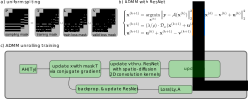
\includegraphics[width=\columnwidth]{../figures/fig1.png}
		\caption{The architecture of a variational autoencoder.
		% The latent variable ($\mathbf{z}$) is sampled from
		}
		% \caption{\textbf{(A)} The architecture of a variational autoencoder.
		% 	\textbf{(B)} An illustration of the joint $k$-$q$-slice forward operator
		% 	for multi-band multi-shot DWI acquisition.
		% 	$[x, y, z, q]$ denotes the shape of input DWI ($\mathbf{\tilde{x}}$),
		% 	with $x$ and $y$ as the image size, $z$ as the number of slices,
		% 	and $q$ as the number of diffusion encodings.
		% 	The operator outputs multi-dimensional $k$-space with the shape $[x, y, 1, c, q, s]$,
		% 	with $c$ as the number of receiver coils, $s$ as the number of shots.}
		\label{FIG:MODEL_VAE}
	\end{figure}

	\subsection{Multi-Band Multi-Shot DWI Acquisition \& Modeling}

	Our previous work \cite{tan_2024_naviepi} demonstrated
	the joint $k$-$q$-slice forward operator
	for multi-band multi-shot NAViEPI DWI acquisition.
	This operator can be understood as
	an extended sensitivity encoding (SENSE) operator \cite{pruessmann_2001_gsense},
	which maps the multi-slice multi-diffusion-weighted images ($\mathbf{\tilde{x}}$)
	to their corresponding $k$-space,
	\begin{equation}
		\mathcal{A}(\mathbf{\tilde{x}}) = \mathbf{P \Sigma \Theta F S \Phi} \mathbf{\tilde{x}}
		\label{EQU:FWD}
	\end{equation}
	Here, the images $\mathbf{\tilde{x}}$ are point-wise multiplied
	with the pre-computed shot-to-shot phase variation maps ($\mathbf{\Phi}$)
	and coil sensitivity maps ($\mathbf{S}$).
	The output images are then converted to $k$-space
	via two-dimensional fast Fourier transform ($\mathbf{F}$),
	point-wise multiplied with the multi-band phases ($\mathbf{\Theta}$),
	summed along the slice dimension ($\mathbf{\Sigma}$),
	and then multiplied by the $k$-space undersampling mask ($\mathbf{P}$).

	With the operator $\mathcal{A}$, the joint reconstruction reads,
	\begin{equation}
		\argmin_{\mathbf{\tilde{x}}} \norm{\mathbf{y} - \mathcal{A}(\mathbf{\tilde{x}})}_2^2 + \lambda \mathcal{R}(\mathbf{\tilde{x}})
		\label{EQU:INV}
	\end{equation}
	where $\mathbf{y}$ is the measured $k$-space data.
	The first term in \cref{EQU:INV} presents data consistency, and
	the second term presents the regularization function $\mathcal{R}(\tilde{x})$
	with the regularization strength $\lambda$.
	When using the Tikhonov regularization,
	i.e.~$\mathcal{R}(\mathbf{\tilde{x}}) = \norm{\mathbf{\tilde{x}}}_2^2$,
	\cref{EQU:INV} can be solved via the conjugate gradient (CG) method.

	\subsection{Variational Autoencoder (VAE)}

	Autoencoders comprise an encoder and a decoder, connected through a latent space.
	Conventional autoencoders have no regularization
	on the latent space.
	Consequently, the learned latent space lacks meaningful
	and structural representation.
	To allow for dimension reduction while keeping the major part of
	the data structure,
	Kingma and Welling \cite{kingma_2014_vae} proposed
	the variational autoencoder (VAE), as shown in \cref{FIG:MODEL_VAE}.
	In VAE, the encoder maps each diffusion-weighted signal
	into a Gaussian distribution ($\mathcal{N}(\mu, \sigma)$) within the latent space.
	The latent variable ($\mathbf{z}$) is sampled according to the encoded distribution.
	The decoder then maps the latent variable to the input space.
	The training of a VAE uses the Huber loss together with the Kullback-Leibler Divergence (KL-D).
	The Huber loss minimizes the difference between the input and the output,
	whereas KL-D minimizes the approximate posterior in latent space and
	the exact posterior (assumed to be Gaussian distribution).


	\subsection{Algorithm Unrolling for Deep Image Reconstruction}

	Algorithm unrolling has been an emerging technique
	in solving \cref{EQU:INV} combining with deep neural networks.
    Algorithm unrolling consists of two ingredients.
	First, it learns a regularization function
	via deep neural networks.
	Second, it is constrained
	by the data-consistency term,
	i.e., the forward pass of the estimate $\mathcal{A} (\mathbf{\tilde{x}})$
	must be close to the measured data $\mathbf{y}$.
    By mapping the operations used in iterative algorithms
    into networks, unrolled algorithms can be trained with data
    and achieve much faster inference
    than conventional iterative algorithms \cite{monga_2021_algunroll}.
    Further, recent developments have shown that
    the operations used in compressed sensing MRI,
    i.e., sparsifying transformation and soft thresholding,
    can be learned via neural networks.
    For instance, Hammernik et al.~\cite{hammernik_2018_varnet}
    proposed to unroll the gradient descent algorithm
    with a learned neural network
    (e.g.~U-net \cite{ronneberger_2015_unet})
    as the regularization function.
    Aggarwal et al.~\cite{aggarwal_2018_modl} proposed to
    unroll the alternating minimization algorithm
    with a learned residual denoising network \cite{he_2016_resnet}
    as regularization.

	% \subsubsection{Variational Network (VarNet)}
	% The unrolling update rule in VarNet \cite{hammernik_2018_varnet} reads
	% \begin{equation} \label{EQU:VarNet_Upd}
	% 	\left\{\begin{aligned}
	% 		\mathbf{z}^{(k)} &= \mathbf{\tilde{x}}^{(k)} - \lambda \cdot \mathcal{A}^H \Big( \mathcal{A} (\mathbf{\tilde{x}}^{(k)}) - \mathbf{y} \Big) \\
	% 		\mathbf{\tilde{x}}^{(k+1)} &= \mathbf{z}^{(k)} - \mathcal{N}_{\theta} (\mathbf{z}^{(k)})
	% 	\end{aligned}\right.
	% \end{equation}
	% with $k$ being the iteration (cascade) step.
	% The regularization is given as a neural network $\mathcal{N}_\theta$.
	% To learn the parameters $\theta$ and the gradient step size $\lambda$,
	% the loss function in VarNet is
	% \begin{equation}
	% 	\argmin_{(\theta, \lambda)} \mathcal{L} (\mathbf{x}_{\text{ref}}, \mathbf{\tilde{x}}^{(K)}) = \norm{\mathbf{\tilde{x}}^{(K)} - \mathbf{x}_{\text{ref}}}_2^2
	% 	\label{EQU:VarNet_Loss}
	% \end{equation}
	% where $\mathbf{\tilde{x}}^{(K)}$ is the estimate after $K$ iterations,
	% and $\mathbf{x}_{\text{ref}}$ denotes fully-sampled reference images.

	% \subsubsection{Model-based deep learning architecture for inverse problems (MoDL)}
	% MoDL \cite{aggarwal_2018_modl} tends to learn a denoising regularization,
	% and redefines \cref{EQU:INV} as
	% \begin{equation}
	% 	\argmin_{\mathbf{\tilde{x}}} \norm{\mathbf{y} - \mathcal{A}(\mathbf{\tilde{x}})}_2^2 + \lambda \norm{ \mathbf{\tilde{x}} - \mathcal{D}_{\omega}(\mathbf{\tilde{x}}) }_2^2
	% 	\label{EQU:DINV}
	% \end{equation}
	% which is solved by the alternating minimization,
	% \begin{equation} \label{EQU:MoDL_Upd}
	% 	\left\{\begin{aligned}
	% 		\mathbf{z}^{(k)} &= \mathcal{D}_{\omega} (\mathbf{\tilde{x}}^{(k)}) \\
	% 		\mathbf{\tilde{x}}^{(k+1)} &= \argmin_{\mathbf{x}} \norm{\mathbf{y} - \mathcal{A}(\mathbf{x})}_2^2 + \lambda \norm{ \mathbf{x} - \mathbf{z}^{(k)} }_2^2
	% 	\end{aligned}\right.
	% \end{equation}
	% where the second minimization problem is solved by CG.
	% MoDL shares weights among iterations, and thus the loss function reduces to
	% only one set of model parameters.
	% Both VarNet and MoDL require reference images,
	% and thus fall into the category of supervised learning.

	% In practice, it is challenging to acquire fully-sampled reference images.
	% To enable deep neural network training without fully sampled reference data,
	% Yaman et al.~\cite{yaman_2020_ssdu} proposed self-supervised learning via data undersampling (SSDU).
	% In SSDU, the undersampled data is partitioned into two disjoint sets,
	% one for the data-consistency term, and another for the loss function calculation.
	% Thus, the sampling mask $\mathbf{P}$ splits,
	% \begin{equation}
	% 	\mathbf{P} = \Theta ~\cup~ \Lambda
	% \end{equation}
	% SSDU follows the alternating update scheme in MoDL,
	% and such a splitting leads to two modifications in training.
	% First, the $k$-space data and the forward model in \cref{EQU:MoDL_Upd} is masked as
	% $\mathbf{y}_{\Theta}$ and $\mathcal{A}_{\Theta}$, respectively.
	% Second, the loss function is computed in $k$-space,
	% \begin{equation}
	% 	\argmin_{(\theta, \lambda)} \mathcal{L} (\mathbf{y}_{\Lambda}, \mathcal{A}_{\Lambda}(\mathbf{\tilde{x}}^{(K)}))
	% 	\label{EQU:SSDU_Loss}
	% \end{equation}
	% where a normalized $\ell_1$-$\ell_2$ loss is used \cite{yaman_2020_ssdu}.
	% Further, Yaman et al.~\cite{yaman_2022_zs} proposed subject-specific zero-shot learning,
	% where one single scan data is partitioned into three disjoint sets,
	% two used to enforce data consistency and to update loss,
	% and the last served as self-validation to allow for early stopping.

	% The regularization function in \cref{EQU:INV} can be nonlinear,
	% e.g.~the sparsity \cite{lustig_2007_cs} or the low-rankness \cite{liang_2007_psf} constraint.
	% In this scenario, algorithms such as
	% the fast iterative shrinkage thresholding (FISTA) \cite{beck_2009_fista}
	% and the alternating direction method of multipliers (ADMM) \cite{boyd_2010_admm}
	% are often employed.
	% These algorithms consist of a substep that transforms $\mathbf{\tilde{x}}$
	% to a sparsifying domain or a specialized matrix format
	% (e.g., the spatial-diffusion matrix in our previous work \cite{tan_2024_naviepi})
	% and then performs nonlinear thresholding to promote sparsity or low-rankness.
	% This substep shares similarities to deep neural networks,
	% and inspires the seminal work on algorithm unrolling
	% by Gregor and LeCun \cite{gregor_2010_algunroll}.
	% Instead of a hand-crafted regularization function,
	% algorithm unrolling learns deep \textit{prior}
	% via the use of deep neural networks as the regularization function.
	% This enables the learning of true image \textit{prior} during the training process
	% and much faster inference than iterative reconstruction with hand-crafted regularization functions.
	% An excellent review of algorithm unrolling
	% has been provided by Monga et al.~\cite{monga_2021_algunroll}.

	% In the area of image reconstruction for accelerated MRI,

    \subsection{Self-Supervised Learning for Image Reconstruction}

    It is difficult to acquire fully-sampled data
    for supervised learning in many MRI applications,
    e.g., dynamic imaging and diffusion-weighted imaging.
    To address this challenge, Yaman et al.~\cite{yaman_2020_ssdu}
    proposed self-supervised learning via data undersampling (SSDU),
    which learns the regularization function in \cref{EQU:INV}
    by splitting available undersampled data into two disjoint sets,
    one of which is used in the data consistency term and
    another used for the training loss function.
    The training of SSDU requires large undersampled data sets.
    To close the domain gap between training and test data,
    Yaman et al.~\cite{yaman_2022_zs} proposed
    scan-specific zero-shot self-supervised learning (ZSSSL),
    which splits a single data set into three disjoint sets
    for the data consistency term and the loss calculation during training,
    and for validation, respectively.
    ZSSSL has been adopted for multi-contrast image reconstruction
    \cite{heydari_2024_jmaple}.

	% ============================== %
	\section{Methods}

    \newcolumntype{a}{p{0.36\columnwidth}}
    \newcolumntype{b}{p{0.20\columnwidth}}
    \begin{table}
        \centering
        \caption{NAViEPI acquisition protocols}
        \label{TAB:ACQ}
        \begin{tabular}{a | b b}
            \toprule
            \textbf{Protocol} & \textbf{\#1} & \textbf{\#2} \\
            \hline
            Diffusion mode & \multicolumn{2}{c}{MDDW} \\
            Diffusion scheme & \multicolumn{2}{c}{monopolar} \\
            Diffusion direction & \multicolumn{2}{c}{$20$} \\
            $b$-value (\si{s/mm^2}) & \multicolumn{2}{c}{$1000$} \\
            $b_0$ & \multicolumn{2}{c}{$1$} \\
            FOV (\si{\square\mm}) & \multicolumn{2}{c}{$200$} \\
            Matrix size & $200 \times 200$ & $286 \times 286$ \\
            In-plane resolution (\si{\square\mm}) & $1.0 \times 1.0$ & $0.7 \times 0.7$ \\
            Slice thickness (\si{\mm}) & $1.0$ & $0.7$ \\
            Slices & $141$ & $176$ \\
            Navigator & No & Yes \\
            Shots & $4$ & $3$ \\
            TR (\si{\ms}) & $7700$ & $16200$ \\
            TE (\si{\ms}) & $67$ & $58/98.3$ \\
            ESP (\si{\ms}) & $1.02$ & $1.17$ \\
            Bandwidth (\si{Hz/Pixel}) & $1086$ & $972$ \\
            Partial Fourier & $6/8$ & $5/8$ \\
            Acceleration & $1 \times 3$ & $2 \times 2$ \\
            Acquisition (\si{\minute}) & $10:42$ & $17:30$ \\
            \bottomrule
        \end{tabular}
    \end{table}

	\subsection{Data Acquisition}

    \cref{TAB:ACQ} lists two acquisition protocols implemented on
	a clinical \SI{7}{\tesla} MR system
	(MAGNETOM Terra, Siemens Healthineers, Erlangen, Germany)
	with a 32-channel head coil (Nova Medical, Wilmington, MA, USA)
	and the XR-gradient system
	(maximum gradient strength \SI{80}{\milli\tesla/\meter} and
	a peak slew rate \SI{200}{\tesla/\meter/\second}).
    The first protocol employed in-plane fully-sampled four-shot EPI
    and thus supplied ground truth data for the validation
    of our proposed methods.
    The second protocol implemented mesoscale \SI{0.7}{mm}
    isotropic resolution based on NAViEPI
    with both in-plane and slice acceleration as 2.
    Two volunteers with written informed consent
	approved by the local ethics committee
	participated in this study.

    \subsection{Image Reconstruction via ADMM Unrolling}

    We employed the ADMM unrolling
    to solve the self-supervised learning reconstruction
    in \cref{EQU:INV}. The update rule of ADMM unrolling reads
	\begin{equation} \label{EQU:ADMM}
		\left\{\begin{aligned}
			\mathbf{\tilde{x}}^{(k+1)} &= \argmin_{\mathbf{x}} \norm{\mathbf{y} - \mathcal{A}(\mathbf{x})}_2^2 + \rho/2 \norm{ \mathbf{x} - \mathbf{v}^{(k)} + \mathbf{u}^{(k)}}_2^2 \\
			\mathbf{v}^{(k+1)} &= (\lambda/\rho) \cdot \mathcal{D}_{\omega} (\mathbf{\tilde{x}}^{(k+1)} + \mathbf{u}^{(k)}) \\
			\mathbf{u}^{(k+1)} &= \mathbf{u}^{(k)} + \mathbf{\tilde{x}}^{(k+1)} - \mathbf{v}^{(k+1)}
		\end{aligned}\right.
	\end{equation}
    ADMM updates the variables $\mathbf{\tilde{x}}$, $\mathbf{v}$,
    and $\mathbf{u}$ in an alternating scheme.
    It splits the unrolled reconstruction into three steps,
    as shown in \cref{EQU:ADMM}.
    The updating step for $\mathbf{\tilde{x}}$ is solved by
    conjugate gradient,
    the variable $\mathbf{v}$ is then updated
    via the forward pass of the neural network $\mathcal{D}_{\omega}$
    with the input as the sum of current estimates
    of $\mathbf{\tilde{x}}$ and $\mathbf{u}$,
    and eventually the variable $\mathbf{u}$ is updated
    based on current estimates of all variables.

    The index $k$ in \cref{EQU:ADMM} denotes the unrolling iteration,
    and $\mathcal{D}_{\omega}$ denotes the residual network
    parameterized by $\omega$.

	\subsection{Latent Space Embedded Zero-Shot Learning}

    ZSSSL partitions the undersampled data into three sets,
    so the sampling mask ($\mathbf{P}$) becomes
    $\mathbf{P} = \mathbf{P}_1 \cup \mathbf{P}_2 \cup \mathbf{P}_3$.
    Here, $\mathbf{P}_1$ is used for the data consistency term
    during training,
    which modifies the $\mathbf{\tilde{x}}$ update step
    in \cref{EQU:ADMM} as
    $\mathbf{\tilde{x}}^{(k+1)} = \argmin_{\mathbf{x}} \norm{\mathbf{P}_1 \mathbf{y} - \mathbf{P}_1 \mathcal{A}(\mathbf{x})}_2^2 + \rho/2 \norm{ \mathbf{x} - \mathbf{v}^{(k)} + \mathbf{u}^{(k)}}_2^2$.
    Given the estimated $\mathbf{\tilde{x}}$,
    $\mathbf{P}_2$ is then used to define the training loss function:
    \begin{equation}
        \label{EQU:LOSS}
        \mathcal{L}(\mathbf{P}_2 \mathbf{y}, \mathbf{P}_2 \mathcal{A}(\mathbf{\tilde{x}}))
    \end{equation}
    which is computed from
    the mixed-$\ell^1$-$\ell^2$ norm of the two inputs
    \cite{yaman_2020_ssdu}.
    $\mathbf{P}_3$ is used to compute the validation loss.
    When the validation loss is consecutively smaller than
    the training loss for 12 times,
    the training process will be stopped.
    After training, the undersampled data set is used for inference.



	% ============================== %
	\section{Results}

	\subsection{VAE enables robust \& accurate learning of DWI signal}

	\subsection{Zero-shot learning enables motion-robust DWI}

	\subsection{Zero-shot learning: model generalization}

	\subsection{VAE modeling with zero-shot learning reconstruction}


	% ============================== %
	\section{Discussion}


	% ============================== %
	\section{Conclusion}


	% ============================== %
	% \section*{Acknowledgment}

	% Z.~Tan thanks to Ms.~Soundarya Soundarresan for
	% her work and discussion on denoising autoencoder,
	% and to Dr.~Xiaoqing Wang for
	% the discussion on self-supervised learning.

	% ============================== %
	\bibliographystyle{IEEEtran}
	\bibliography{../../ref/ref}

\end{document}
